\section{Results}

% TODO: Formatting.
\subsection{Delta Method}
Accuracy from 0 opponents to 10 opponents on PAN2013 dataset 1.
0.44943
0.58235
0.60910
0.62022
0.62719
0.63191
0.63134
0.63550
0.63966
0.63752
0.64191

Accuracy from 0 opponents to 10 opponents on PAN2013 dataset 2.
0.49606
0.57818
0.60133
0.61212
0.61267
0.61748
0.62259
0.62590
0.62708
0.63212
0.62960


Accuracy from 0 opponents to 10 opponents on PAN2015 dataset.
0.50000
0.56170
0.55540
0.54199
0.54089
0.53580
0.52620
0.52650
0.52000
0.51490
0.51500

\begin{figure}
    \centering
    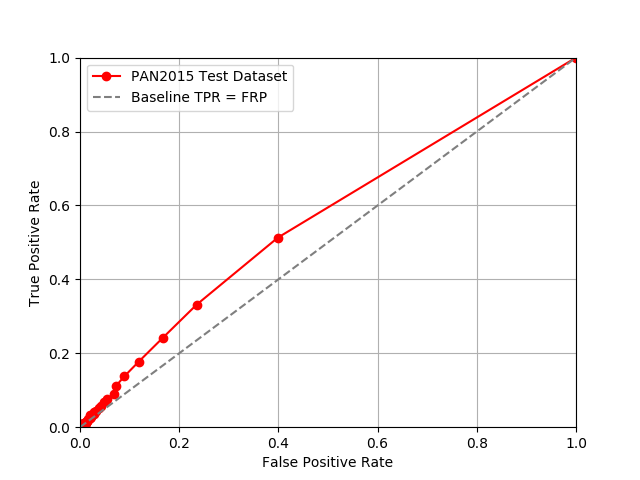
\includegraphics[width=.7\textwidth]{./pictures/delta_method_roc.png}
    \caption{The ROC curve of the delta method with number of opposing authors
    varying from 0 to 10 using the two test datasets for PAN2013 and the test
    dataset for PAN2015.}
    \label{fig:delta_method_roc}
\end{figure}

\subsection{Generalizing Random Forest}

\subsection{Extended Delta}

\subsection{Author Specific SVM}
% SVM performs well on binary authorship problems Abbasi & Chen, 2008; Zheng et al., 2006
% from https://pdfs.semanticscholar.org/5c2b/6876df693e096c6c150a5b0d2a2c05043003.pdf
